\section{Methodology and Results}
\label{sec:experiments}
We begin by using \RPCholesky\ to approximate Gaussian kernel matrices. Given a dataset $D = \{\bx_1, \ldots, \bx_n\}$, the associated $n\times n$ Gaussian kernel matrix $\bK$ is defined by
\[\bK(i, j) = \exp\left(-\frac{1}{2\sigma}\|\bx_i - \bx_j\|^2\right)\]
where the parameter $\sigma > 0$ is called the \textit{bandwidth} of the kernel. The purpose of this study is to understand the Frobenius error of \RPCholesky\ on real-world datasets.

\subsection{Implementation}
The full source code for our implementation and experiments can be found at \href{\GitHubURL}{\GitHubURL}.

\subsection{Relative error comparison}
First, we reproduce a subset of rows from Table 1 of \cite{chen_randomly_2025}, which compares \RPCholesky\ against the greedy sampling method and optimal rank-$k$ approximation. We then repeat these experiments for the Frobenius norm. In all experiments, we measure the \textit{relative error} of the low-rank approximation $\hat\bA$. The relative trace and Frobenius errors are given by
\[\eta_{*} = \frac{\tr(\bA - \hat\bA)}{\tr(\bA)}\qquad\qquad\eta_{F} = \frac{\|\bA - \hat\bA\|_F}{\|\bA\|_F},\]
respectively. The results are recorded in Table \ref{tab:rel-error1000}.
\begin{table}[H]
\centering
\begin{adjustbox}{max width=\textwidth}
\begin{tabular}{wl{3.6cm}cccccc}
\toprule
dataset & & $\eta_\ast$ & & & $\eta_F$ & \\
\cmidrule(lr){2-4}
\cmidrule(lr){5-7}
& Greedy & \RPCholesky & Opt & Greedy & \RPCholesky & Opt \\
\midrule
yolanda & 2.07e-1 & \textbf{1.40e-1} & 8.71e-2 & 4.64e-2 & \textbf{6.30e-3} & 3.15e-3 \\
mnist\_784 & 1.70e-1 & \textbf{1.09e-1} & 5.96e-2 & 2.53e-2 & \textbf{4.95e-3} & 1.97e-3 \\
jannis & 1.27e-1 & \textbf{1.09e-1} & 5.42e-2 & 1.16e-2 & \textbf{6.52e-3} & 2.16e-3 \\
volkert & 6.09e-2 & \textbf{4.31e-2} & 2.06e-2 & 8.15e-3 & \textbf{2.26e-3} & 7.16e-4 \\
creditcard & 4.36e-2 & \textbf{2.32e-2} & 9.87e-3 & 1.04e-2 & \textbf{1.60e-3} & 5.04e-4 \\
hls4ml\_lhc\_jets\_hlf & 6.62e-5 & \textbf{4.47e-5} & 1.07e-5 & 1.27e-5 & \textbf{4.77e-6} & 7.97e-7 \\
\bottomrule
\end{tabular}
\end{adjustbox}
\caption{Relative trace and Frobenius errors of rank-1000 greedy and \RPCholesky\ methods when used to approximate a Gaussian kernel matrix. Each dataset is pruned to $10^4$ points and standardized, and we report the median across 10 trials. The error of the optimal rank-1000 approximation is included for reference.}
\label{tab:rel-error1000}
\end{table}

\begin{figure}[H]
    \centering
    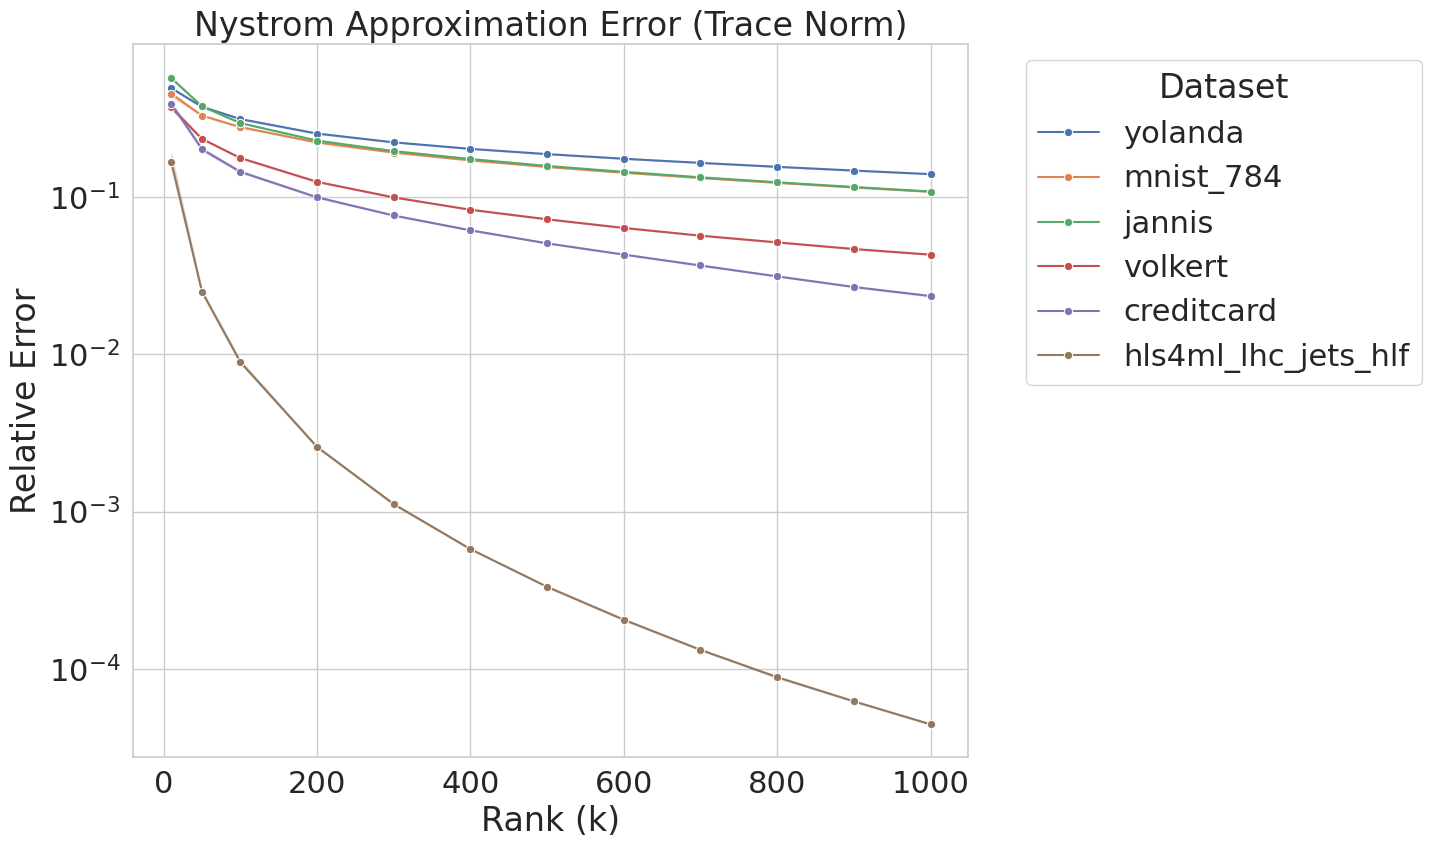
\includegraphics[width=0.8\linewidth]{images/rpcholesky_tr_error.png}
    \caption{Relative trace error vs approximation rank when \RPCholesky\ is used to approximate a Gaussian kernel matrix. Each dataset is trimmed to $10^4$ points and standardized. The bandwidth is set to $\sigma = \sqrt{d}$ for each dataset, where $d$ is the number of features. The plot depicts mean and 95\% confidence interval across 10 trials for each value of $k$.}
    \label{fig:rpcholesky_rel_tr}
\end{figure}

\begin{figure}[H]
    \centering
    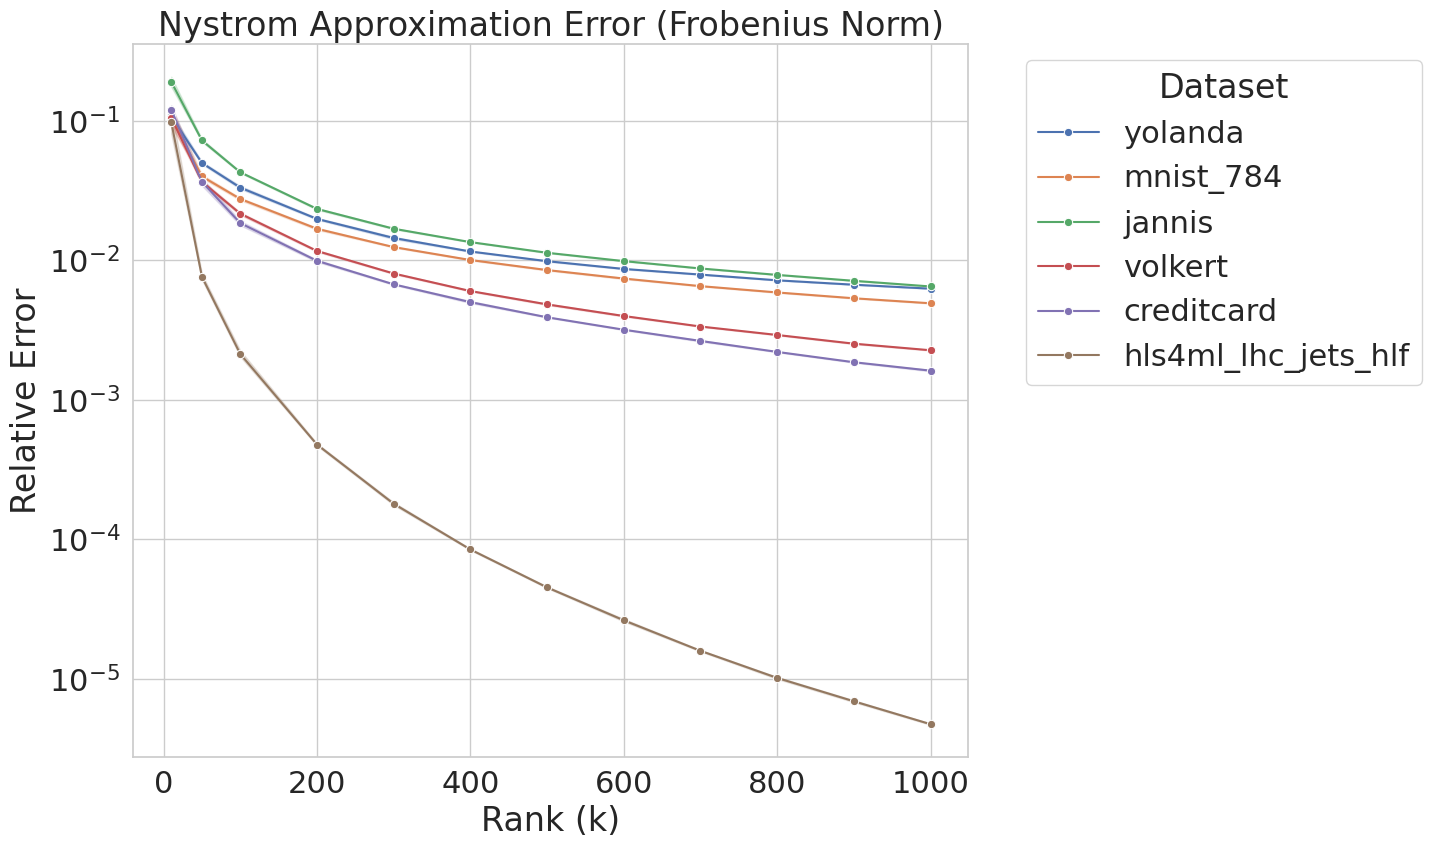
\includegraphics[width=0.8\linewidth]{images/rpcholesky_fro_error.png}
    \caption{Relative Frobenius error vs approximation rank when \RPCholesky\ is used to approximate a Gaussian kernel matrix. Each dataset is trimmed to $10^4$ points and standardized. The bandwidth is set to $\sigma = \sqrt{d}$ for each dataset, where $d$ is the number of features. The plot depicts mean and 95\% confidence interval across 10 trials for each value of $k$.}
    \label{fig:rpcholesky_rel_fro}
\end{figure}

\begin{figure}[H]
    \centering
    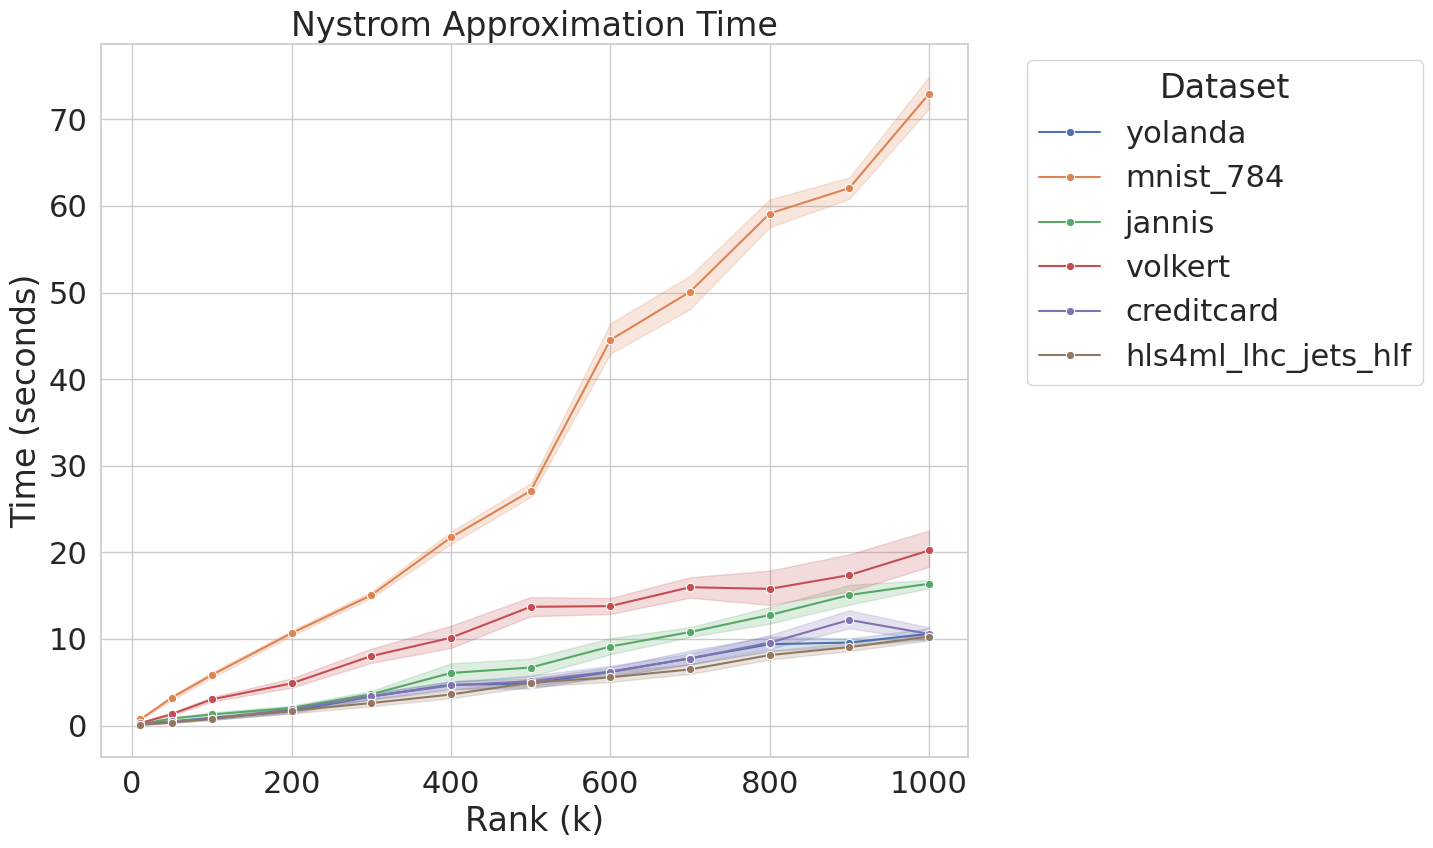
\includegraphics[width=0.8\linewidth]{images/rpcholesky_time.png}
    \caption{Computation time vs approximation rank when \RPCholesky\ is used to approximate a Gaussian kernel matrix. Each dataset is trimmed to $10^4$ points and standardized. The bandwidth is set to $\sigma = \sqrt{d}$ for each dataset, where $d$ is the number of features. The plot depicts mean and 95\% confidence interval across 10 trials for each value of $k$.}
    \label{fig:rpcholesky_time}
\end{figure}

\subsection{Empirical Nystr\"om lower bound}
Theorem \ref{thm:rpc-error} offers a theoretical guarantee on the minimum Nystr\"om approximation rank $k$ required to ensure near-optimal approximation error. In this section, we offer an empirical lower bound based on our Gaussian kernel experiments. 

Let $r$ be a positive integer and $S$ be a subset of column indices. We define $\gamma_{r}(S)$ as
\[
\gamma_{r}(S) := \frac{\|\bA-\bA\gen{S}\|^2}{\|\bA-\bA_r\|^2}\tag{$\ast$}
\]
For a fixed $r$, we are interested in finding the smallest Nystr\"om approximation rank $k$ required to match the optimal rank-$r$ approximation:
\[
\min\{k\geq 1 : \E[\gamma_r(S)] \geq 1+\varepsilon\}
\]
where the expectation is taken over randomized choices for $S$ using a fixed column selection method, e.g., uniform or \RPCholesky. In Figure \ref{fig:k-vs-r}, we plot this value for $S$ produced by the greedy and \RPCholesky\ methods.

\begin{figure}[H]
    \centering
    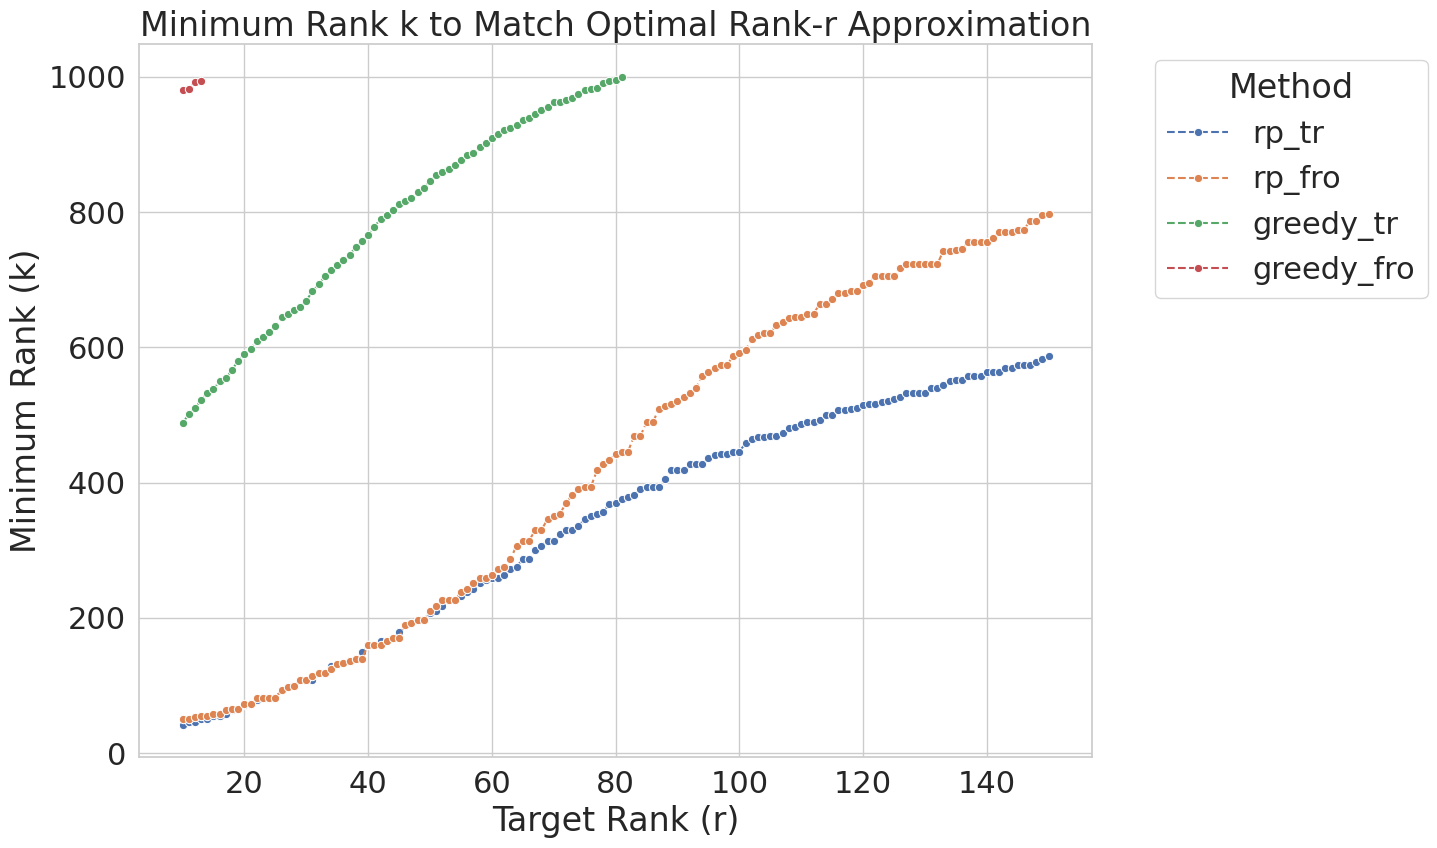
\includegraphics[width=0.98\linewidth]{images/min_k_to_opt_r_threshold1.png}
    \caption{Smallest Nystr\"om approximation rank $k$ required to match optimal rank-$r$ approximation error on the \texttt{yolanda} dataset.}
    \label{fig:k-vs-r}
\end{figure}

Our empirical data suggests that \RPCholesky\ produces a good approximation with respect to the Frobenius norm. If this is the case, can we prove a relative error guarantee for \RPCholesky\ in the Frobenius norm? Theorem~\ref{thm:rpc-frobenius-error-lower-bound} shows that there are worst-case matrices for which \RPCholesky\ cannot find a good approximation.

\begin{theorem}
    \label{thm:rpc-frobenius-error-lower-bound}
    
    % Fix $r\geq 1$ and $\epsilon > 0$. There exists a psd matrix $\bA$ for which the Nystr\"om approximation $\bA\gen{S}$ produced by $\RPCholesky$ satisfies
    % \[\E\left[\|\bA - \bA\gen{S}\|_F^2\right] > (1+\epsilon)\cdot \|\bA -
    %     \llbracket\bA\rrbracket_r\|^2_F\]
    % for all $|S| < r/\epsilon$.
    Fix $r\in\N$ and $c \geq 1$. For $n$ sufficiently large, there exists a psd matrix $\bA\in\R^{n\times n}$ for which the Nystr\"om approximation $\bA\gen{S}$ produced by $\RPCholesky$ satisfies
    \[\E\left[\|\bA - \bA\gen{S}\|_F^2\right] >c\cdot \|\bA -
        \bA_r\|^2_F\]
    for all $|S| < \sqrt{n}/(4c)$.
\end{theorem}

\begin{proof}
    We produce $\bA$ directly. Consider the matrix
    % Consider the $n\times n$ matrix
    % \[\bA = 
    % \begin{pmatrix}
    %     \underbrace{\begin{matrix}
    %     \bJ & \\
    %     & \ddots \\
    %     & &\bJ \\
    %     \end{matrix}}_{\text{$m$ times}}\\
    %     && 1 & \\
    %     && & \ddots \\
    %     && & & 1 \\
    % \end{pmatrix}\]

    \begin{equation} 
    \label{eq:rpcholesky-worst-case}
    \bA = 
    \begin{pmatrix}
        \underbrace{\begin{matrix}
        1 & \cdots & 1 \\
        \vdots& \ddots &\vdots\\
        1 & \cdots & 1 \\
        \end{matrix}}_{\text{$m$}}\\
        && 1 & \\
        && & \ddots \\
        && & & 1 \\
    \end{pmatrix}
    \end{equation}

    The optimal rank-1 approximation is spanned by any of the first $m$ columns of $\bA$, with error 
    \[\delta := \|\bA - \bA_1\|^2_F = n-m.\]
    
   Suppose \RPCholesky\ selects $k$ columns. The diagonal entries of $\bA$ have equal weight, so \RPCholesky\ chooses each column with equal probability. The number of optimal columns selected by \RPCholesky\ follows a hypergeometric distribution, 
   \[X\sim\Hypergeometric(n,m,k).\]
   In particular, the probability that none of the optimal columns are chosen is
   \[
       p := \Pr[X = 0] = \prod_{i=0}^{k-1}\left(1-\frac{m}{n-i}\right).
   \]

   We obtain a lower bound for $p$ as follows:
    \begin{align*}
        p &= \prod_{i=0}^{k-1}\left(1-\frac{m}{n-i}\right)\\
        &= \exp\left(\sum_{i=0}^{k-1}\log\left(1-x_i\right)\right)\qquad x_i=\frac{m}{n-i} \in (0, 1)\\
        &\geq \exp\left(-\sum_{i=0}^{k-1}\frac{m}{n-m-i}\right)\qquad\text{using $\log(1-x_i)\geq -\frac{x_i}{1-x_i}$}\\
        &\geq \exp\left(-\frac{km}{n-m-k}\right).
    \end{align*}
    If in addition we have $k < \sqrt{n}/(4c)$ and $m = c\sqrt{n}$, then 
    \begin{align*}
        n-m-k&\geq n-2m\\
        &\geq \frac{n}{2}\qquad\text{for $n\geq 16c^2$}
    \end{align*}
    and hence
    \begin{align*}
        p &\geq \exp\left(-\frac{km}{n-m-k}\right)\\
        &\geq \exp\left(-1/2\right)\\
        & > 1/2.
    \end{align*}
    
    By inspection, we see that the error of the rank-$k$ \RPCholesky\ approximation satisfies
   \[\|\bA - \bA\gen{S}\|^2_F\geq \begin{cases}
       m^2 +\delta-k&\text{with probability $p$}\\
       \delta-k+1 &\text{with probability $1-p.$}
   \end{cases}\]

   Thus,
   \begin{align*}
       \E\left[\|\bA - \bA\gen{S}\|^2_F\right]&\geq p(m^2+\delta-k)\\
       &> \frac{1}{2}\cdot \left(c^2n-k+\delta\right)\\
       &\geq \frac{1}{2}\cdot \delta(c^2+1)\\
       & \geq c\cdot \delta \qquad\text{for all $c\geq 1$}\\
       & \geq c\cdot \|\bA - \bA_r\|^2_F.
   \end{align*}

    Choosing $n$ large enough so that 
    \[n\geq 16c^2\]
    completes the proof.
    % where each $\bJ$ is the $\sqrt{n}\times \sqrt{n}$ all-ones matrix.
\end{proof}


\begin{figure}[H]
    \centering
    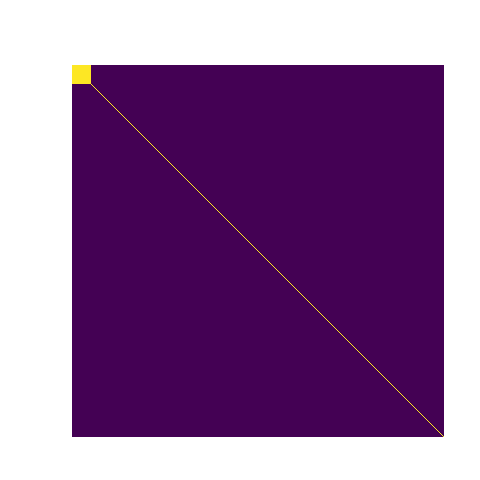
\includegraphics[width=0.60\linewidth]{images/rpcholesky_hard_matrix_c5_p0.0001_kernel_heatmap.png}
    \caption{Gaussian kernel matrix for the geometric dataset at $N=10^4$, $d=100$, and $c = 500$.}
    \label{fig:geom-hard}
\end{figure}

We conclude by giving a geometric interpretation of the hard matrices identified in Theorem~\ref{thm:rpc-frobenius-error-lower-bound}. Consider forming a dataset with $N$ points of dimension $d$ containing
\begin{enumerate}
    \item $c\sqrt{N}$ points drawn from a spherical Gaussian distribution centered at the origin with covariance matrix $p\bI$, and
    \item $N - c\sqrt{N}$ points corresponding to the vertices of the $d$-dimensional hypercube of width 2 centered at the origin.
\end{enumerate}
Then the Gaussian kernel matrix of this dataset resembles the matrices of Theorem~\ref{thm:rpc-frobenius-error-lower-bound}. This resemblance is illustrated in Figure~\ref{fig:geom-hard}.

% \begin{proposition} \label{prop:rpc-hard}
%     \RPCholesky\ error guarantee fails on the gaussian (inner product) kernel matrix of the dataset above?
% \end{proposition}


\subsection{An algorithm for Frobenius-error approximation}
Here, we propose a new pivot selection method that avoids the worst-case matrices in (\ref{eq:rpcholesky-worst-case}). As the proof of Theorem~\ref{thm:rpc-frobenius-error-lower-bound} suggests, sampling columns proportional to the diagonal entries will miss large hidden columns. Instead, we sample a reasonably large principal submatrix and choose the largest column, picking up approximately large columns in the original matrix. 

\begin{algorithm}[ht]
\DontPrintSemicolon
    \label{alg:rpc2}
    \caption{\RPCholesky2}
    $\bR\gets \bA - \hat\bA$\;
    $J\gets \left\{j_1, j_2,\ldots, j_{c\sqrt{n}}\right\}$ with $j_k\sim P: p_i = \bR_{ii}/\tr(R)$\;
    $\bD\gets \sqrt{\diag\left(\frac{1}{{p_1}},\ldots, \frac{1}{{p_{\sqrt{n}}}}\right)}$\;
    $\bS\gets \bD\bR(J, J)\bD$\;
    \Return $\argmax_i \|\bS\bar s_i\|_2^2\qquad \bar s_i := \bS_i/\|\bS_i\|.$
\end{algorithm}

% \begin{proposition}
%     Let $\bM$ be a real matrix. The column of $\bM$ which yields the best rank-1 approximation is given by 
%     \[\argmax_i \|\bM \bar{m_i}\|^2\qquad \bar{m_i} = \frac{\bM_i}{\|\bM_i\|}.\]
% \end{proposition}


\subsection{Numerical experiments}
Table~\ref{tab:rpc2-rel-error1000} Compares the relative error of $\RPCholesky2$ against $\RPCholesky$. 

\begin{figure}[H]
    \centering
    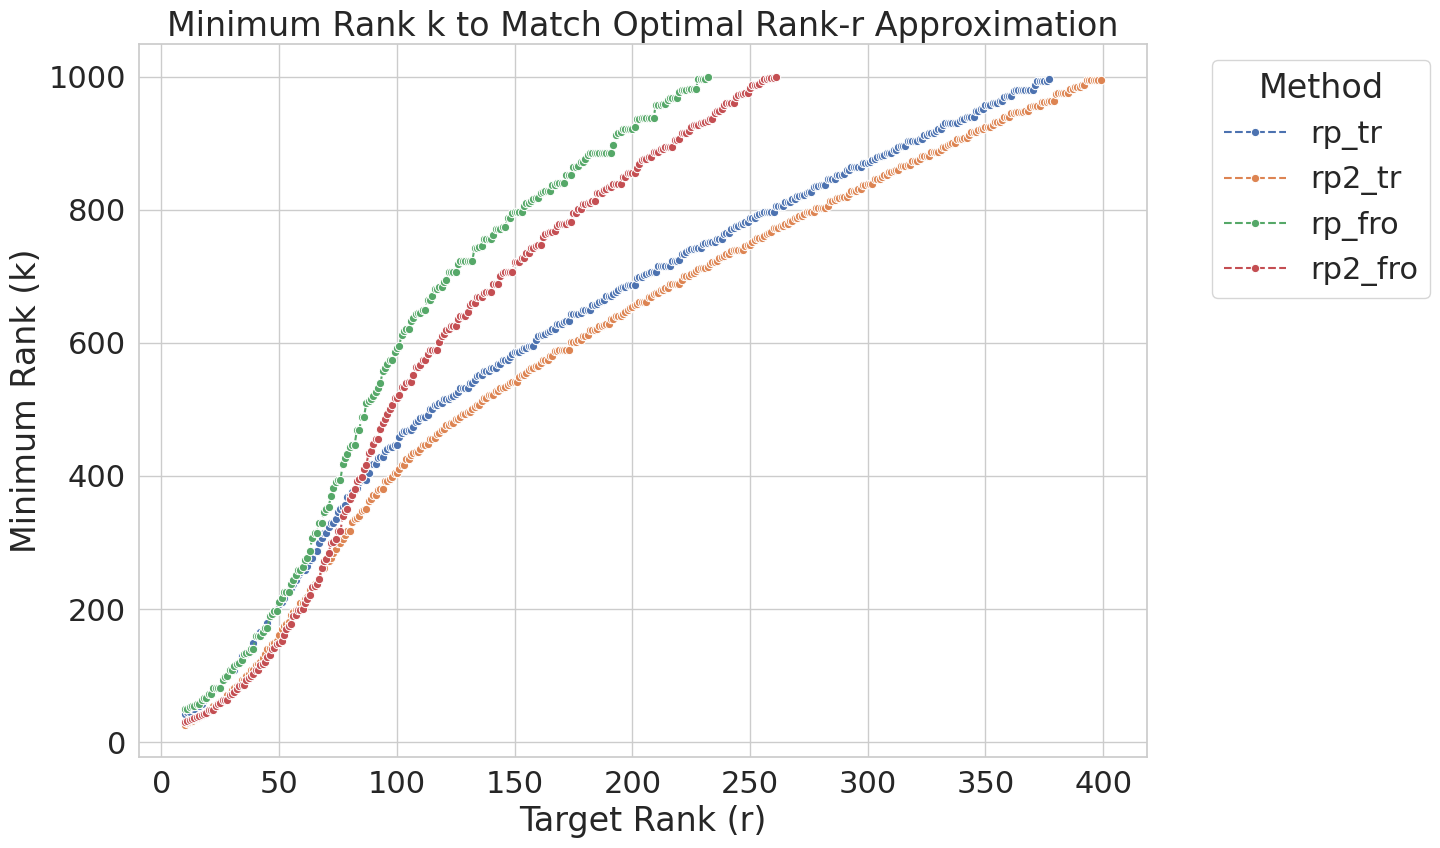
\includegraphics[width=0.90\linewidth]{images/min2_k_to_opt_r_threshold1.png}
    \caption{Empirically, \RPCholesky2 outperforms \RPCholesky\ on both Frobenius and trace norms.}
    \label{fig:rpc2-vs-rpc}
\end{figure}

\begin{table}[H]
\centering
\begin{adjustbox}{max width=\textwidth}
\begin{tabular}{wl{3.6cm}cccccc}
\toprule
dataset & & $\eta_\ast$ & & & $\eta_F$ & \\
\cmidrule(lr){2-4}
\cmidrule(lr){5-7}
& \RPCholesky2 & \RPCholesky & Opt & \RPCholesky2 & \RPCholesky & Opt \\
\midrule
yolanda & \textbf{1.38e-1} & 1.40e-1 & 8.71e-2 & \textbf{6.02e-3} & 6.30e-3 & 3.15e-3 \\
mnist\_784 & \textbf{1.04e-1} & 1.09e-1 & 5.96e-2 & \textbf{4.67e-3} & 4.95e-3 & 1.97e-3 \\
jannis & \textbf{1.07e-1} & 1.09e-1 & 5.42e-2 & \textbf{6.27e-3} & 6.52e-3 & 2.16e-3 \\
volkert & \textbf{4.07e-2} & 4.31e-2 & 2.06e-2 & \textbf{2.09e-3} & 2.26e-3 & 7.16e-4 \\
creditcard & \textbf{2.08e-2} & 2.32e-2 & 9.87e-3 & \textbf{1.39e-3} & 1.60e-3 & 5.04e-4 \\
hls4ml\_lhc\_jets\_hlf & \textbf{3.98e-5} & 4.47e-5 & 1.07e-5 & \textbf{4.01e-6} & 4.77e-6 & 7.97e-7 \\
\bottomrule
\end{tabular}
\end{adjustbox}
\caption{Relative trace and Frobenius error comparison between rank-1000 \RPCholesky\ and \RPCholesky2 methods when used to approximate a Gaussian kernel matrix. Each dataset is pruned to $10^4$ points and standardized, and we report the median across 10 trials. The error of the optimal rank-1000 approximation is included for reference.}
\label{tab:rpc2-rel-error1000}
\end{table}

\begin{figure}[H]
    \centering
    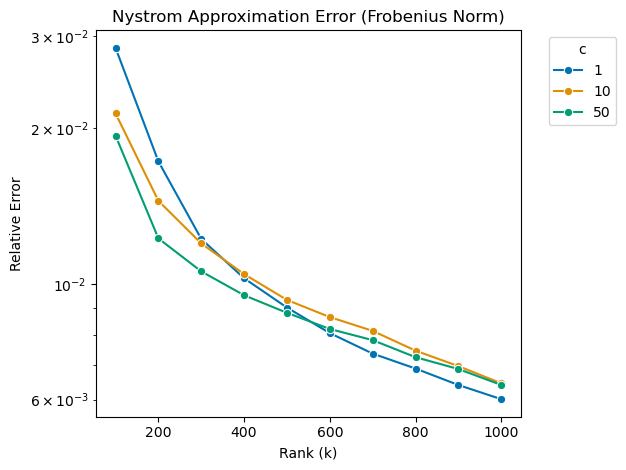
\includegraphics[width=0.75\linewidth]{images/rpc3_yolanda_fro_error_c.png}
    \caption{Relative error of $\RPCholesky2$ on the \texttt{yolanda} dataset with varied choices of $c$, where $c\sqrt{n}$ is the number of indices to take for the principal submatrix at every step.}
    \label{fig:placeholder}
\end{figure}

% \begin{figure}[H]
%     \centering
%     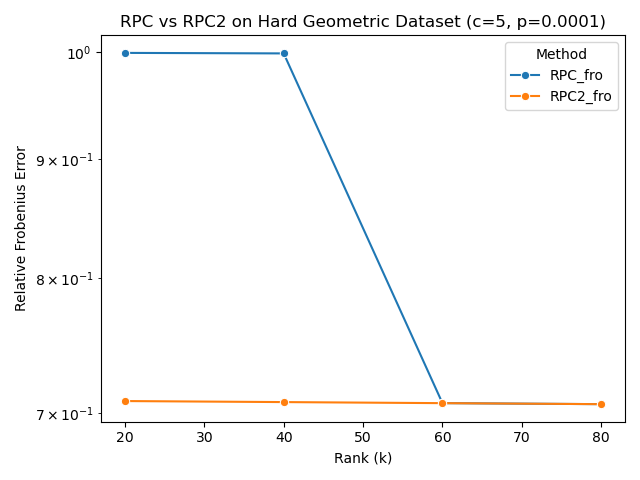
\includegraphics[width=0.85\linewidth]{images/rpcholesky_hard_case_c5_p0.0001.png}
%     \caption{$\RPCholesky$ vs $\RPCholesky2$ on the hard geometric dataset for $N = 10^4$ and $d=100$.}
%     \label{fig:rpc-hard}
% \end{figure}



% \todo[inline,color=orange!60]{I noticed that taking $\argmax \|c_i\|$ over columns of the residual matrix yields the same performance.}



% \todo[inline,color=orange!60,caption={}]{\textbf{Aaron:}
% \begin{enumerate}
%     \item Look into Column Subset Selection problem
%     \item Proving theoretical guarantee
%     \begin{enumerate}
%         \item \cite{deshpande_adaptive_2006} adaptive sampling; c.f. Theorem 3 and Corollary 1. Approach: prove bound for first iteration of algorithm, then proceed by induction. Maybe we can do similar?
%         \item \cite{wang_improving_2013} lower bound on adaptive sampling for Nystr\"om method, c.f. Appendix C.2
%     \end{enumerate}
% \end{enumerate}
% }

% \newpage
% \subsection{Equivalence between RPC and Adaptive Sampling}
% \cite{deshpande_adaptive_2006} details a procedure for adaptive sampling as follows\\
% \begin{algorithm}[H]
% \DontPrintSemicolon
% \caption{Adaptive Sampling}
% \label{alg:adaptivesampling}
% \KwIn{Matrix B $\in \mathbb{R}^{m \times n}$}
% \KwOut{Selected index set S
% }
% $R \gets B$\;
% $S \gets \emptyset$\;
% \Repeat{stopping criterion met}{
%     Sample $i$ with probability $p_i \propto \dfrac{R_{ii}}{\operatorname{tr}(R)} = \dfrac{\|r_i\|_2^2}{\|R\|_F^2}$\;
%     $S \gets S \cup \{i\}$\;
%     $R \gets B - P_{BS}B$\;
% }
% \end{algorithm}
% $P_{BS}$ is the projection matrix onto the selected columns of $B$. It's explicit computation is given by $UU^T$, where $U$ is the matrix containing the left singular vectors of $BS$. To recap,
% \begin{algorithm}
% \DontPrintSemicolon
% \caption{RPCholesky}
% \label{alg:rpcholesky}
% \KwIn{Positive semi-definite matrix $A \in \mathbb{R}^{n \times n}$}
% \KwOut{Selected index set $S$}
% $R \gets A$\;
% $S \gets \emptyset$\;
% \Repeat{stopping criterion met}{
%     Sample $i$ with probability $p_i = \dfrac{R_{ii}}{\operatorname{tr}(R)}$\;
%     $S \gets S \cup \{i\}$\;
%     $R \gets A - A S (S^\top A S)^{-1} S^\top A$\;
% }
% \end{algorithm}

% \newpage
% \begin{theorem}
%     \label{thm:adaptive-sampling}
%     (Deshpande et al. \cite{deshpande_adaptive_2006}) Any $m\times n$ matrix $\bB$ contains a subset $S$ of $4k/\epsilon + 2k\log(k+1)$ rows such that there is a matrix $\tilde\bB_k$ of rank at most $k$ whose rows lie in $\matspan(S)$ and \todo{this is not quite the statement I want}
%     \[\|\bB - \tilde\bB_k\|^2_F\leq(1+\epsilon)\|\bB - \opt{\bB}_k\|^2_F.\]
% \end{theorem}

% \begin{proof}
%     (Theorem \ref{thm:rpc-error} implies Theorem \ref{thm:adaptive-sampling}). Let $\bA = \bB^\top\bB$. We show the following:
%     \begin{enumerate}
%         \item Let $S$ be a column selection matrix, $\bR_\bB = \bB - \bP_{\bB\bS}\bB$ and $\bR_\bA = \bA - \bA\gen{S}$. Then,
%         \[\bR_\bB^\top\bR_\bB = \bR_\bA.\]
%         \item The index set $S_A$ produced by RPCholesky on $\bA$ follows the same distribution as $S_B$ produced by adaptive sampling on $\bB$.
%     \end{enumerate}

%     In particular, applying (1) to Theorem 5 yields the desired result:
%     \begin{align*}
%         (1+\epsilon)\tr(\bA - \opt{\bA}_r)&\geq \tr(\bA-\bA\gen{S})\\
%         &=\tr(\bR_\bB^\top \bR_\bB)\\
%         &= \|\bB-\bP_{\bB\bS}\bB\|^2_F.
%     \end{align*}
    
%     \vspace{1em}
%     (1) Compute directly:
%     \begin{align*}
%         \bR_{\bB}^\top\bR_{\bB} &= (\bB-\bP_{\bB\bS}\bB)^\top(\bB-\bP_{\bB\bS}\bB)\\
%         &= \bB^\top\bB - \bB^\top\bP_{\bB\bS}\bB - \bB^\top\bP_{\bB\bS}^\top\bB +\bB^\top\bP_{\bB\bS}^\top\bP_{\bB\bS}\bB\\
%         &=\bB^\top\bB - \bB^\top\bP_{\bB\bS}\bB\qquad\text{$\bP_{\bB\bS}$ is symmetric, idempotent}\\
%         &= \bA - \bB^\top\bB\bS(\bS^\top\bB^\top\bB\bS)^{-1}\bS^\top\bB^\top\bB\\
%         &= \bA - \bA\bS(\bS^\top\bA\bS)^{-1}\bS^\top\bA\\
%         &= \bA - \bA\gen{S}.
%     \end{align*}

%     (2) Let $\bR_\bA^i, \bR_\bB^i$ denote the residual matrices after $i$ iterations of RPCholesky and adaptive sampling, respectively. We inductively compare the index sampling distributions and show that they are equal at every step. Initially $\bR_\bA^0 = \bA$, $\bR_\bB^0 = \bB$, and $\bR_\bA^0 = \bR_\bB^{0\top}\bR_\bB^0$ with $S_A^0 = S_B^0 = \varnothing$.

%     Suppose $\bR_\bA^i = \bR_\bB^{i\top}\bR_\bB^i$ at step $i$ of RPCholesky and adaptive sampling. Then RPCholesky samples index $j$ with probability 
%     \begin{align*}
%         p_{j,A} &= \frac{\bR_{\bA}^i(j,j)}{\tr(\bR_{\bA}^i)}\\[5pt]
%         &=\frac{\bR_\bB^{i\top}\bR_\bB^i(j,j)}{\tr(\bR_\bB^{i\top}\bR_\bB^i)}\\[5pt]
%         &=\frac{\|\bR_\bB^i(:,j)\|^2_2}{\|\bR_\bB^{i\top}\bR_\bB^i\|_F^2} = p_{j,B}.
%     \end{align*}
%     Moreover, if RPCholesky and adaptive sampling choose the same index, then $S_A^{i+1} = S_B^{i+1}$. Apply (1) to find that $\bR_\bA^{i+1} = \bR_\bB^{i+1\,\top}\bR_\bB^{i+1}$. We are done by induction.
% \end{proof}

% \newpage
% \begin{lemma}
%     Let $\bA$ be an $n\times n$ PSD matrix and suppose $\bU$ satisfies $\bA = \bU^\top\bU$. For any matrix $\bOmega\in\R^{n\times k}$, let $\bR_{\bA\gen{\bOmega}}$ denote the Nystr\"om residual $\bA - \bA\gen{\bOmega}$ and let $\bR_{\bU\bOmega} = \bU - \bP_{\bU\bOmega}\bU$.

%     \begin{enumerate}
%         \item $\bA\gen{\bOmega} = \bU\bP_{\bU\bOmega}\bU$
%         \item $\bR_{\bA\gen{\bOmega}} = \bR_{\bU\bOmega}^\top\bR_{\bU\bOmega}$
%     \end{enumerate}
% \end{lemma}

\subsection{Nystr\"om lower bound for the Frobenius norm}
\label{sec:nystrom-lb}
\begin{theorem}
    \label{thm:nystrom-frobenius-lb}
    (Nystr\"om lower bound). For all $\alpha \geq 1$, there exist PSD matrices $\bA\in\R^{n\times n}$ such that \textbf{any} rank-$k$ column Nystr\"om approximation with 
    \[ k \leq \sqrt{n/(2\alpha)}\]
    has error $\|\bA - \bA\gen{S}\|^2_F > \alpha\cdot \|\bA - \bA_1\|^2_F$.
\end{theorem}


\begin{proof}
Let $\bA = \bI_n + \delta\bJ_n$ for some $\delta \geq 1$. The eigenvalues of $\bA$ are 
\[\lambda_1 = 1+n\delta \qquad \lambda_2 = 1\qquad\cdots\qquad \lambda_n = 1.\]
The first eigenvector of $\bA$ is $\bu_1 = (1/\sqrt n)\mathbf{1}$, and the best rank-1 approximation to $\bA$ is therefore given by
\[\bA_1 = (1 + n\delta)\bu_1\bu_1^\top = \left(\frac{1}{n}+\delta\right)\bJ_n \qquad 1 + n\delta \geq 1\]
with approximation error
\begin{align*}
    \|\bA - \bA_1\|^2_F = \sum_{i=2}^n\lambda_i^2 =n-1.\tag{$\ast$}
\end{align*}

On the other hand, suppose we choose $k$ columns of $\bA$ to compute the Nystr\"om approximation $\bA\gen{S}$. Without loss of generality, we can take the first $k$ columns, i.e., set $S = [k]$. With $d = n-k$, partition $\bA$ into blocks as follows:
\[\bA = \begin{pmatrix}
    \bA_{kk} & \bA_{kd}\\
    \bA_{dk} & \bA_{dd}
\end{pmatrix}\]
where 
\[\bA_{kk} = \bI_k + \delta\bJ_k\qquad \bA_{dk} = \bA_{kd}^\top = \delta\mathbf{1}_{d\times k}\qquad \bA_{dd} = \bI_d + \delta\bJ_d.\]

\vspace{1em}
The Nystr\"om approximation in block form is given by
\[\bA\gen{S} = \begin{pmatrix}
    \bA_{kk}\\
    \bA_{dk}
\end{pmatrix} \bA_{kk}^{-1}\begin{pmatrix}
    \bA_{kk}\\
    \bA_{dk}
\end{pmatrix}^\top = \begin{pmatrix}
    \bA_{kk} & \bA_{kd}\\
    \bA_{dk} & \bA_{dk}\bA_{kk}^{-1}\bA_{kd}
\end{pmatrix}.\]
In particular,
\[\bA - \bA\gen{S} = \begin{pmatrix}
    0 & 0\\
    0 & \bA_{dd} - \bA_{dk}\bA_{kk}^{-1}\bA_{kd}
\end{pmatrix}\]
so the error of the Nystr\"om approximation is
\[\|\bA - \bA\gen{S}\|^2_F = \|\bA_{dd} - \bA_{dk}\bA_{kk}^{-1}\bA_{kd}\|^2_F.\]
Now, set $\bR := \bA_{dd} - \bA_{dk}\bA_{kk}^{-1}\bA_{kd}$ and compute directly:
\begin{align*}
    \bR &= \bA_{dd}- \bA_{dk}\left(\bI_k + \delta \mathbf{1}_k\mathbf{1}_k^\top\right)^{-1}\bA_{kd}\\
    &=\bA_{dd}- \bA_{dk}\left(\bI_k - \frac{\delta \mathbf{1}_k\mathbf{1}_k^\top}{1+\delta \mathbf{1}_k^\top\mathbf{1}_k}\right)\bA_{kd}\qquad\text{(Sherman-Morrison)}\\[5pt]
    &=\bA_{dd}-\delta^2 \mathbf{1}_{d\times k}\left(\bI_k - \frac{\delta }{1+k\delta}\mathbf{1}_{k\times k}\right)\mathbf{1}_{k\times d}\\
    &=\bA_{dd}-\delta^2 \mathbf{1}_{d\times k}\left(\mathbf{1}_{k\times d} - \frac{k\delta}{1+k\delta}\mathbf{1}_{k\times d}\right)\\
    &=\bA_{dd}-\delta^2 \mathbf{1}_{d\times k}\left(\frac{1}{1+k\delta}\mathbf{1}_{k\times d}\right)\\
    &=\bA_{dd} - \frac{k\delta^2}{1+k\delta}\mathbf{1}_{d\times d}\\
    &= \bI_d + \delta\mathbf{1}_{d\times d} - \frac{k\delta^2}{1+k\delta}\mathbf{1}_{d\times d}\\
    &= \bI_d + \frac{\delta}{1+k\delta}\mathbf{1}_{d\times d}.\\
\end{align*}

Based on the above characterization, the eigenvalues of $\bR$ are
\[\lambda_1 = 1+\frac{d\delta}{1+k\delta} = \frac{1 + n\delta}{1 + k\delta}\qquad\lambda_2 = 1\qquad\cdots\qquad\lambda_d = 1\]
Thus, the approximation error satisfies
\begin{align*}
    \|\bA - \bA\gen{S}\|^2_F &= \sum_{i=1}^d \lambda_i^2\\
    &\geq \lambda_1^2 = \left(\frac{1+n\delta}{1+k\delta}\right)^2\\
    &\geq \frac{n^2\delta^2}{2 k^2\delta^2}\qquad\text{for $\delta$ sufficiently large}\\
    &\geq \alpha\cdot n\qquad\text{for $k \leq \sqrt{n/(2\alpha)}$}\\
    & > \alpha\cdot(n-1) \\
    &= \alpha\cdot \|\bA-\bA_1\|^2_F
    % & \geq \alpha\cdot \|\bA-\opt{\bA}_r\|^2_F
\end{align*}
as required.
\end{proof}
% \todo[inline,color=orange!40]{For $\|\bA - \bA\gen{S}\|^2_F > \eta\cdot \|\bA - \opt{\bA}_r\|^2_F$, we should be able to modify the proof to show that $k > \sqrt{n/\rho\eta}$ is necessary.}